\documentclass[twoside]{book}

% Packages required by doxygen
\usepackage{calc}
\usepackage{doxygen}
\usepackage{graphicx}
\usepackage[utf8]{inputenc}
\usepackage{makeidx}
\usepackage{multicol}
\usepackage{multirow}
\usepackage{textcomp}
\usepackage[table]{xcolor}

% Font selection
\usepackage[T1]{fontenc}
\usepackage{mathptmx}
\usepackage[scaled=.90]{helvet}
\usepackage{courier}
\usepackage{amssymb}
\usepackage{sectsty}
\renewcommand{\familydefault}{\sfdefault}
\allsectionsfont{%
  \fontseries{bc}\selectfont%
  \color{darkgray}%
}
\renewcommand{\DoxyLabelFont}{%
  \fontseries{bc}\selectfont%
  \color{darkgray}%
}

% Page & text layout
\usepackage{geometry}
\geometry{%
  a4paper,%
  top=2.5cm,%
  bottom=2.5cm,%
  left=2.5cm,%
  right=2.5cm%
}
\tolerance=750
\hfuzz=15pt
\hbadness=750
\setlength{\emergencystretch}{15pt}
\setlength{\parindent}{0cm}
\setlength{\parskip}{0.2cm}
\makeatletter
\renewcommand{\paragraph}{%
  \@startsection{paragraph}{4}{0ex}{-1.0ex}{1.0ex}{%
    \normalfont\normalsize\bfseries\SS@parafont%
  }%
}
\renewcommand{\subparagraph}{%
  \@startsection{subparagraph}{5}{0ex}{-1.0ex}{1.0ex}{%
    \normalfont\normalsize\bfseries\SS@subparafont%
  }%
}
\makeatother

% Headers & footers
\usepackage{fancyhdr}
\pagestyle{fancyplain}
\fancyhead[LE]{\fancyplain{}{\bfseries\thepage}}
\fancyhead[CE]{\fancyplain{}{}}
\fancyhead[RE]{\fancyplain{}{\bfseries\leftmark}}
\fancyhead[LO]{\fancyplain{}{\bfseries\rightmark}}
\fancyhead[CO]{\fancyplain{}{}}
\fancyhead[RO]{\fancyplain{}{\bfseries\thepage}}
\fancyfoot[LE]{\fancyplain{}{}}
\fancyfoot[CE]{\fancyplain{}{}}
\fancyfoot[RE]{\fancyplain{}{\bfseries\scriptsize Generated on Sun Dec 22 2013 03:36:13 for Locaudio by Doxygen }}
\fancyfoot[LO]{\fancyplain{}{\bfseries\scriptsize Generated on Sun Dec 22 2013 03:36:13 for Locaudio by Doxygen }}
\fancyfoot[CO]{\fancyplain{}{}}
\fancyfoot[RO]{\fancyplain{}{}}
\renewcommand{\footrulewidth}{0.4pt}
\renewcommand{\chaptermark}[1]{%
  \markboth{#1}{}%
}
\renewcommand{\sectionmark}[1]{%
  \markright{\thesection\ #1}%
}

% Indices & bibliography
\usepackage{natbib}
\usepackage[titles]{tocloft}
\setcounter{tocdepth}{3}
\setcounter{secnumdepth}{5}
\makeindex

% Hyperlinks (required, but should be loaded last)
\usepackage{ifpdf}
\ifpdf
  \usepackage[pdftex,pagebackref=true]{hyperref}
\else
  \usepackage[ps2pdf,pagebackref=true]{hyperref}
\fi
\hypersetup{%
  colorlinks=true,%
  linkcolor=blue,%
  citecolor=blue,%
  unicode%
}

% Custom commands
\newcommand{\clearemptydoublepage}{%
  \newpage{\pagestyle{empty}\cleardoublepage}%
}


%===== C O N T E N T S =====

\begin{document}

% Titlepage & ToC
\hypersetup{pageanchor=false}
\pagenumbering{roman}
\begin{titlepage}
\vspace*{7cm}
\begin{center}%
{\Large Locaudio }\\
\vspace*{1cm}
{\large Generated by Doxygen 1.8.4}\\
\vspace*{0.5cm}
{\small Sun Dec 22 2013 03:36:13}\\
\end{center}
\end{titlepage}
\clearemptydoublepage
\tableofcontents
\clearemptydoublepage
\pagenumbering{arabic}
\hypersetup{pageanchor=true}

%--- Begin generated contents ---
\chapter{Namespace Index}
\section{Packages}
Here are the packages with brief descriptions (if available)\-:\begin{DoxyCompactList}
\item\contentsline{section}{\hyperlink{namespacelocaudio}{locaudio} }{\pageref{namespacelocaudio}}{}
\item\contentsline{section}{\hyperlink{namespacelocaudio_1_1detectionevent}{locaudio.\-detectionevent} }{\pageref{namespacelocaudio_1_1detectionevent}}{}
\item\contentsline{section}{\hyperlink{namespacelocaudio_1_1triangulation}{locaudio.\-triangulation} }{\pageref{namespacelocaudio_1_1triangulation}}{}
\end{DoxyCompactList}

\chapter{Hierarchical Index}
\section{Class Hierarchy}
This inheritance list is sorted roughly, but not completely, alphabetically\-:\begin{DoxyCompactList}
\item \contentsline{section}{object}{\pageref{classobject}}{}
\begin{DoxyCompactList}
\item \contentsline{section}{locaudio.\-detectionevent.\-Detection\-Event}{\pageref{classlocaudio_1_1detectionevent_1_1DetectionEvent}}{}
\item \contentsline{section}{locaudio.\-point.\-Point}{\pageref{classlocaudio_1_1point_1_1Point}}{}
\end{DoxyCompactList}
\end{DoxyCompactList}

\chapter{Class Index}
\section{Class List}
Here are the classes, structs, unions and interfaces with brief descriptions\-:\begin{DoxyCompactList}
\item\contentsline{section}{\hyperlink{classlocaudio_1_1detectionevent_1_1DetectionEvent}{locaudio.\-detectionevent.\-Detection\-Event} \\*Class which is used to house the detection event }{\pageref{classlocaudio_1_1detectionevent_1_1DetectionEvent}}{}
\item\contentsline{section}{\hyperlink{classlocaudio_1_1api_1_1Locaudio}{locaudio.\-api.\-Locaudio} }{\pageref{classlocaudio_1_1api_1_1Locaudio}}{}
\item\contentsline{section}{\hyperlink{classobject}{object} }{\pageref{classobject}}{}
\item\contentsline{section}{\hyperlink{classlocaudio_1_1point_1_1Point}{locaudio.\-point.\-Point} }{\pageref{classlocaudio_1_1point_1_1Point}}{}
\end{DoxyCompactList}

\chapter{File Index}
\section{File List}
Here is a list of all files with brief descriptions\-:\begin{DoxyCompactList}
\item\contentsline{section}{/\-Users/wallarelvo-\/mac/\-Documents/\-Projects/locaudio/locaudio/\hyperlink{____init_____8py}{\-\_\-\-\_\-init\-\_\-\-\_\-.\-py} }{\pageref{____init_____8py}}{}
\item\contentsline{section}{/\-Users/wallarelvo-\/mac/\-Documents/\-Projects/locaudio/locaudio/\hyperlink{api_8py}{api.\-py} }{\pageref{api_8py}}{}
\item\contentsline{section}{/\-Users/wallarelvo-\/mac/\-Documents/\-Projects/locaudio/locaudio/\hyperlink{config_8py}{config.\-py} }{\pageref{config_8py}}{}
\item\contentsline{section}{/\-Users/wallarelvo-\/mac/\-Documents/\-Projects/locaudio/locaudio/\hyperlink{detectionevent_8py}{detectionevent.\-py} }{\pageref{detectionevent_8py}}{}
\item\contentsline{section}{/\-Users/wallarelvo-\/mac/\-Documents/\-Projects/locaudio/locaudio/\hyperlink{detectionserver_8py}{detectionserver.\-py} }{\pageref{detectionserver_8py}}{}
\item\contentsline{section}{/\-Users/wallarelvo-\/mac/\-Documents/\-Projects/locaudio/locaudio/\hyperlink{fingerprint_8py}{fingerprint.\-py} }{\pageref{fingerprint_8py}}{}
\item\contentsline{section}{/\-Users/wallarelvo-\/mac/\-Documents/\-Projects/locaudio/locaudio/\hyperlink{point_8py}{point.\-py} }{\pageref{point_8py}}{}
\item\contentsline{section}{/\-Users/wallarelvo-\/mac/\-Documents/\-Projects/locaudio/locaudio/\hyperlink{triangulation_8py}{triangulation.\-py} }{\pageref{triangulation_8py}}{}
\end{DoxyCompactList}

\chapter{Namespace Documentation}
\hypertarget{namespacelocaudio}{\section{locaudio Namespace Reference}
\label{namespacelocaudio}\index{locaudio@{locaudio}}
}
\subsection*{Namespaces}
\begin{DoxyCompactItemize}
\item 
\hyperlink{namespacelocaudio_1_1detectionevent}{detectionevent}
\item 
\hyperlink{namespacelocaudio_1_1detectionserver}{detectionserver}
\item 
\hyperlink{namespacelocaudio_1_1point}{point}
\item 
\hyperlink{namespacelocaudio_1_1triangulation}{triangulation}
\end{DoxyCompactItemize}
\subsection*{Variables}
\begin{DoxyCompactItemize}
\item 
string \hyperlink{namespacelocaudio_a08bd2e574ba3b2af29ee1231a056dcc5}{\-\_\-\-\_\-author\-\_\-\-\_\-} = \char`\"{}Alexander Wallar $<$aw204@st-\/andrews.\-ac.\-uk$>$\char`\"{}
\end{DoxyCompactItemize}


\subsection{Variable Documentation}
\hypertarget{namespacelocaudio_a08bd2e574ba3b2af29ee1231a056dcc5}{\index{locaudio@{locaudio}!\-\_\-\-\_\-author\-\_\-\-\_\-@{\-\_\-\-\_\-author\-\_\-\-\_\-}}
\index{\-\_\-\-\_\-author\-\_\-\-\_\-@{\-\_\-\-\_\-author\-\_\-\-\_\-}!locaudio@{locaudio}}
\subsubsection[{\-\_\-\-\_\-author\-\_\-\-\_\-}]{\setlength{\rightskip}{0pt plus 5cm}string locaudio.\-\_\-\-\_\-author\-\_\-\-\_\- = \char`\"{}Alexander Wallar $<$aw204@st-\/andrews.\-ac.\-uk$>$\char`\"{}}}\label{namespacelocaudio_a08bd2e574ba3b2af29ee1231a056dcc5}


Definition at line 2 of file \-\_\-\-\_\-init\-\_\-\-\_\-.\-py.


\hypertarget{namespacelocaudio_1_1api}{\section{locaudio.\-api Namespace Reference}
\label{namespacelocaudio_1_1api}\index{locaudio.\-api@{locaudio.\-api}}
}
\subsection*{Classes}
\begin{DoxyCompactItemize}
\item 
class \hyperlink{classlocaudio_1_1api_1_1Locaudio}{Locaudio}
\end{DoxyCompactItemize}

\hypertarget{namespacelocaudio_1_1config}{\section{locaudio.\-config Namespace Reference}
\label{namespacelocaudio_1_1config}\index{locaudio.\-config@{locaudio.\-config}}
}
\subsection*{Variables}
\begin{DoxyCompactItemize}
\item 
tuple \hyperlink{namespacelocaudio_1_1config_a360c0d0146f0defa6e852b004d834513}{app} = Flask(\-\_\-\-\_\-name\-\_\-\-\_\-)
\item 
tuple \hyperlink{namespacelocaudio_1_1config_ac701fbe139aea54ed29426657c92739e}{detection\-\_\-events} = list()
\item 
int \hyperlink{namespacelocaudio_1_1config_a7a507b1534e99737ed545a117b87313b}{refresh\-\_\-time} = 10
\item 
\hyperlink{namespacelocaudio_1_1config_a6c08de266870244fd753c8dc6047bfec}{reference\-\_\-print} = None
\item 
tuple \hyperlink{namespacelocaudio_1_1config_afc387e694f7bc08bccf873238760ce8e}{position\-\_\-list} = list()
\item 
\hyperlink{namespacelocaudio_1_1config_aa8acdbffcae328560e4231de29c2dc1a}{new\-\_\-data} = False
\end{DoxyCompactItemize}


\subsection{Variable Documentation}
\hypertarget{namespacelocaudio_1_1config_a360c0d0146f0defa6e852b004d834513}{\index{locaudio\-::config@{locaudio\-::config}!app@{app}}
\index{app@{app}!locaudio::config@{locaudio\-::config}}
\subsubsection[{app}]{\setlength{\rightskip}{0pt plus 5cm}tuple locaudio.\-config.\-app = Flask(\-\_\-\-\_\-name\-\_\-\-\_\-)}}\label{namespacelocaudio_1_1config_a360c0d0146f0defa6e852b004d834513}


Definition at line 4 of file config.\-py.

\hypertarget{namespacelocaudio_1_1config_ac701fbe139aea54ed29426657c92739e}{\index{locaudio\-::config@{locaudio\-::config}!detection\-\_\-events@{detection\-\_\-events}}
\index{detection\-\_\-events@{detection\-\_\-events}!locaudio::config@{locaudio\-::config}}
\subsubsection[{detection\-\_\-events}]{\setlength{\rightskip}{0pt plus 5cm}tuple locaudio.\-config.\-detection\-\_\-events = list()}}\label{namespacelocaudio_1_1config_ac701fbe139aea54ed29426657c92739e}


Definition at line 7 of file config.\-py.

\hypertarget{namespacelocaudio_1_1config_aa8acdbffcae328560e4231de29c2dc1a}{\index{locaudio\-::config@{locaudio\-::config}!new\-\_\-data@{new\-\_\-data}}
\index{new\-\_\-data@{new\-\_\-data}!locaudio::config@{locaudio\-::config}}
\subsubsection[{new\-\_\-data}]{\setlength{\rightskip}{0pt plus 5cm}locaudio.\-config.\-new\-\_\-data = False}}\label{namespacelocaudio_1_1config_aa8acdbffcae328560e4231de29c2dc1a}


Definition at line 13 of file config.\-py.

\hypertarget{namespacelocaudio_1_1config_afc387e694f7bc08bccf873238760ce8e}{\index{locaudio\-::config@{locaudio\-::config}!position\-\_\-list@{position\-\_\-list}}
\index{position\-\_\-list@{position\-\_\-list}!locaudio::config@{locaudio\-::config}}
\subsubsection[{position\-\_\-list}]{\setlength{\rightskip}{0pt plus 5cm}tuple locaudio.\-config.\-position\-\_\-list = list()}}\label{namespacelocaudio_1_1config_afc387e694f7bc08bccf873238760ce8e}


Definition at line 12 of file config.\-py.

\hypertarget{namespacelocaudio_1_1config_a6c08de266870244fd753c8dc6047bfec}{\index{locaudio\-::config@{locaudio\-::config}!reference\-\_\-print@{reference\-\_\-print}}
\index{reference\-\_\-print@{reference\-\_\-print}!locaudio::config@{locaudio\-::config}}
\subsubsection[{reference\-\_\-print}]{\setlength{\rightskip}{0pt plus 5cm}locaudio.\-config.\-reference\-\_\-print = None}}\label{namespacelocaudio_1_1config_a6c08de266870244fd753c8dc6047bfec}


Definition at line 10 of file config.\-py.

\hypertarget{namespacelocaudio_1_1config_a7a507b1534e99737ed545a117b87313b}{\index{locaudio\-::config@{locaudio\-::config}!refresh\-\_\-time@{refresh\-\_\-time}}
\index{refresh\-\_\-time@{refresh\-\_\-time}!locaudio::config@{locaudio\-::config}}
\subsubsection[{refresh\-\_\-time}]{\setlength{\rightskip}{0pt plus 5cm}int locaudio.\-config.\-refresh\-\_\-time = 10}}\label{namespacelocaudio_1_1config_a7a507b1534e99737ed545a117b87313b}


Definition at line 8 of file config.\-py.


\hypertarget{namespacelocaudio_1_1detectionevent}{\section{locaudio.\-detectionevent Namespace Reference}
\label{namespacelocaudio_1_1detectionevent}\index{locaudio.\-detectionevent@{locaudio.\-detectionevent}}
}
\subsection*{Classes}
\begin{DoxyCompactItemize}
\item 
class \hyperlink{classlocaudio_1_1detectionevent_1_1DetectionEvent}{Detection\-Event}
\begin{DoxyCompactList}\small\item\em Class which is used to house the detection event. \end{DoxyCompactList}\end{DoxyCompactItemize}

\hypertarget{namespacelocaudio_1_1detectionserver}{\section{locaudio.\-detectionserver Namespace Reference}
\label{namespacelocaudio_1_1detectionserver}\index{locaudio.\-detectionserver@{locaudio.\-detectionserver}}
}
\subsection*{Functions}
\begin{DoxyCompactItemize}
\item 
def \hyperlink{namespacelocaudio_1_1detectionserver_a5191437c6dcef4900a200a7dd115a58a}{post\-\_\-notify}
\end{DoxyCompactItemize}
\subsection*{Variables}
\begin{DoxyCompactItemize}
\item 
tuple \hyperlink{namespacelocaudio_1_1detectionserver_aef3614adbb1729e98db6ad1e92df44aa}{app} = Flask(\-\_\-\-\_\-name\-\_\-\-\_\-)
\end{DoxyCompactItemize}


\subsection{Function Documentation}
\hypertarget{namespacelocaudio_1_1detectionserver_a5191437c6dcef4900a200a7dd115a58a}{\index{locaudio\-::detectionserver@{locaudio\-::detectionserver}!post\-\_\-notify@{post\-\_\-notify}}
\index{post\-\_\-notify@{post\-\_\-notify}!locaudio::detectionserver@{locaudio\-::detectionserver}}
\subsubsection[{post\-\_\-notify}]{\setlength{\rightskip}{0pt plus 5cm}def locaudio.\-detectionserver.\-post\-\_\-notify (
\begin{DoxyParamCaption}
{}
\end{DoxyParamCaption}
)}}\label{namespacelocaudio_1_1detectionserver_a5191437c6dcef4900a200a7dd115a58a}


Definition at line 8 of file detectionserver.\-py.



\subsection{Variable Documentation}
\hypertarget{namespacelocaudio_1_1detectionserver_aef3614adbb1729e98db6ad1e92df44aa}{\index{locaudio\-::detectionserver@{locaudio\-::detectionserver}!app@{app}}
\index{app@{app}!locaudio::detectionserver@{locaudio\-::detectionserver}}
\subsubsection[{app}]{\setlength{\rightskip}{0pt plus 5cm}tuple locaudio.\-detectionserver.\-app = Flask(\-\_\-\-\_\-name\-\_\-\-\_\-)}}\label{namespacelocaudio_1_1detectionserver_aef3614adbb1729e98db6ad1e92df44aa}


Definition at line 4 of file detectionserver.\-py.


\hypertarget{namespacelocaudio_1_1fingerprint}{\section{locaudio.\-fingerprint Namespace Reference}
\label{namespacelocaudio_1_1fingerprint}\index{locaudio.\-fingerprint@{locaudio.\-fingerprint}}
}
\subsection*{Functions}
\begin{DoxyCompactItemize}
\item 
def \hyperlink{namespacelocaudio_1_1fingerprint_aff6c231dfe74871cf275c4b8249fafb2}{get\-\_\-similarity}
\end{DoxyCompactItemize}
\subsection*{Variables}
\begin{DoxyCompactItemize}
\item 
tuple \hyperlink{namespacelocaudio_1_1fingerprint_ad6f4abf7a6777721b881a7f0188afe92}{Reference\-Print} = namedtuple(\char`\"{}Reference\-Print\char`\"{}, \char`\"{}fingerprint radius spl\char`\"{})
\end{DoxyCompactItemize}


\subsection{Function Documentation}
\hypertarget{namespacelocaudio_1_1fingerprint_aff6c231dfe74871cf275c4b8249fafb2}{\index{locaudio\-::fingerprint@{locaudio\-::fingerprint}!get\-\_\-similarity@{get\-\_\-similarity}}
\index{get\-\_\-similarity@{get\-\_\-similarity}!locaudio::fingerprint@{locaudio\-::fingerprint}}
\subsubsection[{get\-\_\-similarity}]{\setlength{\rightskip}{0pt plus 5cm}def locaudio.\-fingerprint.\-get\-\_\-similarity (
\begin{DoxyParamCaption}
\item[{}]{f\-\_\-1, }
\item[{}]{f\-\_\-2}
\end{DoxyParamCaption}
)}}\label{namespacelocaudio_1_1fingerprint_aff6c231dfe74871cf275c4b8249fafb2}


Definition at line 9 of file fingerprint.\-py.



\subsection{Variable Documentation}
\hypertarget{namespacelocaudio_1_1fingerprint_ad6f4abf7a6777721b881a7f0188afe92}{\index{locaudio\-::fingerprint@{locaudio\-::fingerprint}!Reference\-Print@{Reference\-Print}}
\index{Reference\-Print@{Reference\-Print}!locaudio::fingerprint@{locaudio\-::fingerprint}}
\subsubsection[{Reference\-Print}]{\setlength{\rightskip}{0pt plus 5cm}tuple locaudio.\-fingerprint.\-Reference\-Print = namedtuple(\char`\"{}Reference\-Print\char`\"{}, \char`\"{}fingerprint radius spl\char`\"{})}}\label{namespacelocaudio_1_1fingerprint_ad6f4abf7a6777721b881a7f0188afe92}


Definition at line 6 of file fingerprint.\-py.


\hypertarget{namespacelocaudio_1_1point}{\section{locaudio.\-point Namespace Reference}
\label{namespacelocaudio_1_1point}\index{locaudio.\-point@{locaudio.\-point}}
}
\subsection*{Classes}
\begin{DoxyCompactItemize}
\item 
class \hyperlink{classlocaudio_1_1point_1_1Point}{Point}
\end{DoxyCompactItemize}

\hypertarget{namespacelocaudio_1_1triangulation}{\section{locaudio.\-triangulation Namespace Reference}
\label{namespacelocaudio_1_1triangulation}\index{locaudio.\-triangulation@{locaudio.\-triangulation}}
}
\subsection*{Functions}
\begin{DoxyCompactItemize}
\item 
def \hyperlink{namespacelocaudio_1_1triangulation_a4a7017521badc87c46d0b84774d70b2f}{distance\-From\-Sound}
\begin{DoxyCompactList}\small\item\em Determines the distance from a sound given the sound pressure level and a reference sound pressure level with an associated distance. \end{DoxyCompactList}\item 
def \hyperlink{namespacelocaudio_1_1triangulation_ac52a12426ddad7f84fd8fdce6d53a7e0}{distance\-From\-Detection\-Event}
\begin{DoxyCompactList}\small\item\em Given x and y coordinates, this returns the distance to a node\-Event where the node\-Event has attributes, x and y, on the same plane. \end{DoxyCompactList}\item 
def \hyperlink{namespacelocaudio_1_1triangulation_aeda79115af2a41e618d834fe29a63104}{normal\-Distribution}
\begin{DoxyCompactList}\small\item\em This is the normal distribution function. \end{DoxyCompactList}\item 
def \hyperlink{namespacelocaudio_1_1triangulation_af600bbadd299c94825b159b5df236f6f}{position\-Evaluation}
\begin{DoxyCompactList}\small\item\em Evaluation function to deterimine with some weight, where a sound is located in the mesh network of nodes. \end{DoxyCompactList}\item 
def \hyperlink{namespacelocaudio_1_1triangulation_af708227f069b847392f730d13060cce8}{position\-Probability}
\begin{DoxyCompactList}\small\item\em Scales the evaluation function so it returns a probability (i.\-e. \end{DoxyCompactList}\item 
def \hyperlink{namespacelocaudio_1_1triangulation_abd8cf1c3aaf884f1c97cbeb6c853f697}{determine\-Sound\-Position}
\begin{DoxyCompactList}\small\item\em Gets the x and y position of a sound in a mesh network given a set of node events. \end{DoxyCompactList}\item 
def \hyperlink{namespacelocaudio_1_1triangulation_a4e6907d01e9d4a6cd7ba3d7d3a41b3b2}{generate\-Sound\-Position\-Func}
\begin{DoxyCompactList}\small\item\em This is a closure that provides a new function that makes it so the developer does not need to continue passing the r\-Ref, l\-Ref and init\-Guess variables when determining the sound position. \end{DoxyCompactList}\end{DoxyCompactItemize}
\subsection*{Variables}
\begin{DoxyCompactItemize}
\item 
float \hyperlink{namespacelocaudio_1_1triangulation_ac85bcbed961d15baa586ddc0192860bb}{K} = 0.\-7
\begin{DoxyCompactList}\small\item\em Scaling constant to transform a confidence probability into a a standard deviation. \end{DoxyCompactList}\end{DoxyCompactItemize}


\subsection{Function Documentation}
\hypertarget{namespacelocaudio_1_1triangulation_abd8cf1c3aaf884f1c97cbeb6c853f697}{\index{locaudio\-::triangulation@{locaudio\-::triangulation}!determine\-Sound\-Position@{determine\-Sound\-Position}}
\index{determine\-Sound\-Position@{determine\-Sound\-Position}!locaudio::triangulation@{locaudio\-::triangulation}}
\subsubsection[{determine\-Sound\-Position}]{\setlength{\rightskip}{0pt plus 5cm}def locaudio.\-triangulation.\-determine\-Sound\-Position (
\begin{DoxyParamCaption}
\item[{}]{r\-Ref, }
\item[{}]{l\-Ref, }
\item[{}]{init\-Guess, }
\item[{}]{node\-Events}
\end{DoxyParamCaption}
)}}\label{namespacelocaudio_1_1triangulation_abd8cf1c3aaf884f1c97cbeb6c853f697}


Gets the x and y position of a sound in a mesh network given a set of node events. 

In order to establish the x and y positions we need a reference sound pressure level and the distance when this measurement was taken.


\begin{DoxyParams}{Parameters}
{\em r\-Ref} & The reference distance at which the reference sound pressure level was recorded\\
\hline
{\em l\-Ref} & The reference sound pressure level used to determine the distance from the newly measured sound pressure level\\
\hline
{\em init\-Guess} & The initial guess for gradient decent\\
\hline
{\em node\-Events} & The list ofassociated data when a node detects with some confidence that the sound has been identified\\
\hline
\end{DoxyParams}
\begin{DoxyReturn}{Returns}
The x and y position of the sound. 
\end{DoxyReturn}


Definition at line 199 of file triangulation.\-py.



Here is the call graph for this function\-:\nopagebreak
\begin{figure}[H]
\begin{center}
\leavevmode
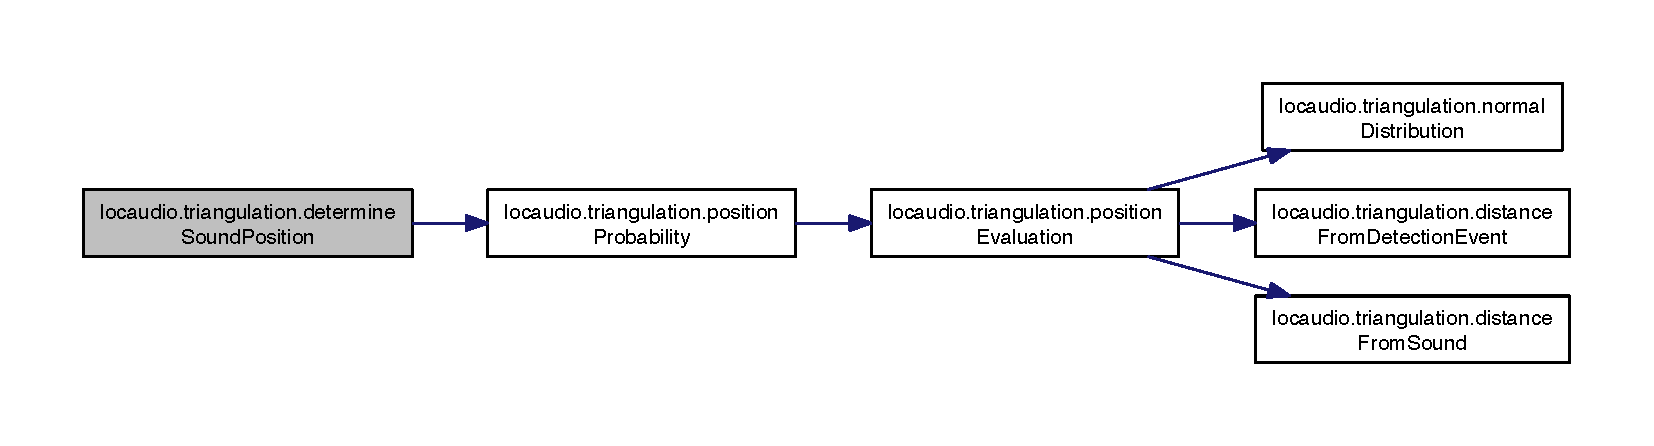
\includegraphics[width=350pt]{namespacelocaudio_1_1triangulation_abd8cf1c3aaf884f1c97cbeb6c853f697_cgraph}
\end{center}
\end{figure}


\hypertarget{namespacelocaudio_1_1triangulation_ac52a12426ddad7f84fd8fdce6d53a7e0}{\index{locaudio\-::triangulation@{locaudio\-::triangulation}!distance\-From\-Detection\-Event@{distance\-From\-Detection\-Event}}
\index{distance\-From\-Detection\-Event@{distance\-From\-Detection\-Event}!locaudio::triangulation@{locaudio\-::triangulation}}
\subsubsection[{distance\-From\-Detection\-Event}]{\setlength{\rightskip}{0pt plus 5cm}def locaudio.\-triangulation.\-distance\-From\-Detection\-Event (
\begin{DoxyParamCaption}
\item[{}]{x, }
\item[{}]{y, }
\item[{}]{node\-Event}
\end{DoxyParamCaption}
)}}\label{namespacelocaudio_1_1triangulation_ac52a12426ddad7f84fd8fdce6d53a7e0}


Given x and y coordinates, this returns the distance to a node\-Event where the node\-Event has attributes, x and y, on the same plane. 


\begin{DoxyParams}{Parameters}
{\em x} & the horizontal location of the node event when the node event was captured\\
\hline
{\em y} & the vertical location of the node event when the node event was captured\\
\hline
{\em node\-Event} & The associated data when a node detects with some confidence that the sound has been identified\\
\hline
\end{DoxyParams}
\begin{DoxyReturn}{Returns}
The distance from a node event given x and y coordinates 
\end{DoxyReturn}


Definition at line 74 of file triangulation.\-py.



Here is the caller graph for this function\-:\nopagebreak
\begin{figure}[H]
\begin{center}
\leavevmode
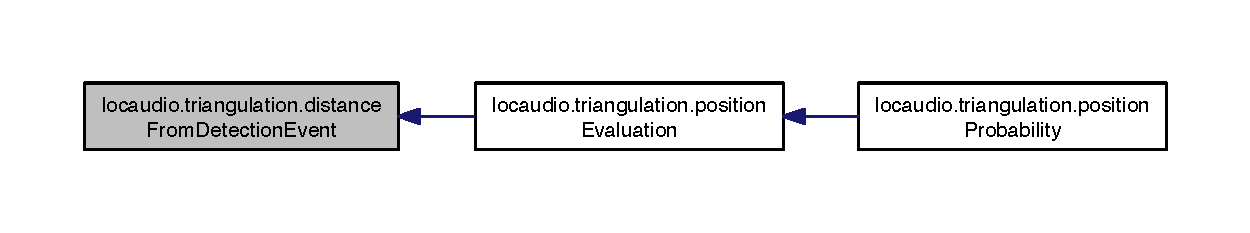
\includegraphics[width=350pt]{namespacelocaudio_1_1triangulation_ac52a12426ddad7f84fd8fdce6d53a7e0_icgraph}
\end{center}
\end{figure}


\hypertarget{namespacelocaudio_1_1triangulation_a4a7017521badc87c46d0b84774d70b2f}{\index{locaudio\-::triangulation@{locaudio\-::triangulation}!distance\-From\-Sound@{distance\-From\-Sound}}
\index{distance\-From\-Sound@{distance\-From\-Sound}!locaudio::triangulation@{locaudio\-::triangulation}}
\subsubsection[{distance\-From\-Sound}]{\setlength{\rightskip}{0pt plus 5cm}def locaudio.\-triangulation.\-distance\-From\-Sound (
\begin{DoxyParamCaption}
\item[{}]{r\-Ref, }
\item[{}]{l\-Ref, }
\item[{}]{l\-Current}
\end{DoxyParamCaption}
)}}\label{namespacelocaudio_1_1triangulation_a4a7017521badc87c46d0b84774d70b2f}


Determines the distance from a sound given the sound pressure level and a reference sound pressure level with an associated distance. 


\begin{DoxyParams}{Parameters}
{\em r\-Ref} & The reference distance at which the reference sound pressure level was recorded\\
\hline
{\em l\-Ref} & The reference sound pressure level used to determine the distance from the newly measured sound pressure level\\
\hline
{\em l\-Current} & Newly measured sound pressure level\\
\hline
\end{DoxyParams}
\begin{DoxyReturn}{Returns}
The predicted radius from a node event that the sound will be located at given the current sound pressure level 
\end{DoxyReturn}


Definition at line 51 of file triangulation.\-py.



Here is the caller graph for this function\-:\nopagebreak
\begin{figure}[H]
\begin{center}
\leavevmode
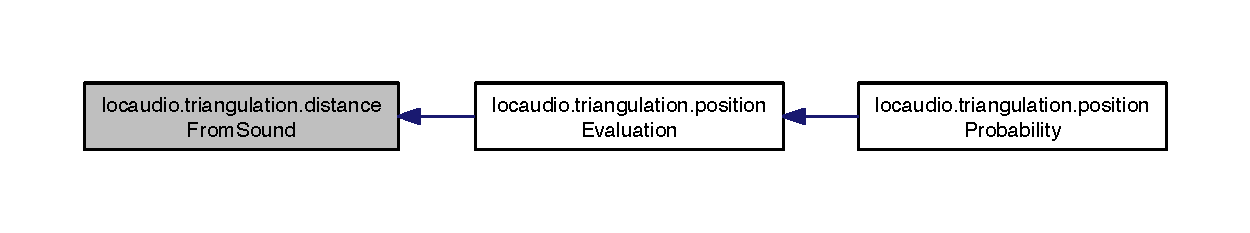
\includegraphics[width=350pt]{namespacelocaudio_1_1triangulation_a4a7017521badc87c46d0b84774d70b2f_icgraph}
\end{center}
\end{figure}


\hypertarget{namespacelocaudio_1_1triangulation_a4e6907d01e9d4a6cd7ba3d7d3a41b3b2}{\index{locaudio\-::triangulation@{locaudio\-::triangulation}!generate\-Sound\-Position\-Func@{generate\-Sound\-Position\-Func}}
\index{generate\-Sound\-Position\-Func@{generate\-Sound\-Position\-Func}!locaudio::triangulation@{locaudio\-::triangulation}}
\subsubsection[{generate\-Sound\-Position\-Func}]{\setlength{\rightskip}{0pt plus 5cm}def locaudio.\-triangulation.\-generate\-Sound\-Position\-Func (
\begin{DoxyParamCaption}
\item[{}]{r\-Ref, }
\item[{}]{l\-Ref, }
\item[{}]{init\-Guess}
\end{DoxyParamCaption}
)}}\label{namespacelocaudio_1_1triangulation_a4e6907d01e9d4a6cd7ba3d7d3a41b3b2}


This is a closure that provides a new function that makes it so the developer does not need to continue passing the r\-Ref, l\-Ref and init\-Guess variables when determining the sound position. 

This is most useful when tracking a sound throughout an enivronment because these parameters will stay constant.


\begin{DoxyParams}{Parameters}
{\em r\-Ref} & The reference distance at which the reference sound pressure level was recorded\\
\hline
{\em l\-Ref} & The reference sound pressure level used to determine the distance from the newly measured sound pressure level\\
\hline
{\em init\-Guess} & The initial guess for gradient decent\\
\hline
\end{DoxyParams}
\begin{DoxyReturn}{Returns}
A function that will use r\-Ref, l\-Ref, and init\-Guess to determine the position of the input sound. The independent variable will become just the node detection events. 
\end{DoxyReturn}


Definition at line 232 of file triangulation.\-py.

\hypertarget{namespacelocaudio_1_1triangulation_aeda79115af2a41e618d834fe29a63104}{\index{locaudio\-::triangulation@{locaudio\-::triangulation}!normal\-Distribution@{normal\-Distribution}}
\index{normal\-Distribution@{normal\-Distribution}!locaudio::triangulation@{locaudio\-::triangulation}}
\subsubsection[{normal\-Distribution}]{\setlength{\rightskip}{0pt plus 5cm}def locaudio.\-triangulation.\-normal\-Distribution (
\begin{DoxyParamCaption}
\item[{}]{x}
\end{DoxyParamCaption}
)}}\label{namespacelocaudio_1_1triangulation_aeda79115af2a41e618d834fe29a63104}


This is the normal distribution function. 


\begin{DoxyParams}{Parameters}
{\em x} & Input for the normal distribution function\\
\hline
\end{DoxyParams}
\begin{DoxyReturn}{Returns}
The resulting value for the probability desnsity function 
\end{DoxyReturn}


Definition at line 92 of file triangulation.\-py.



Here is the caller graph for this function\-:\nopagebreak
\begin{figure}[H]
\begin{center}
\leavevmode
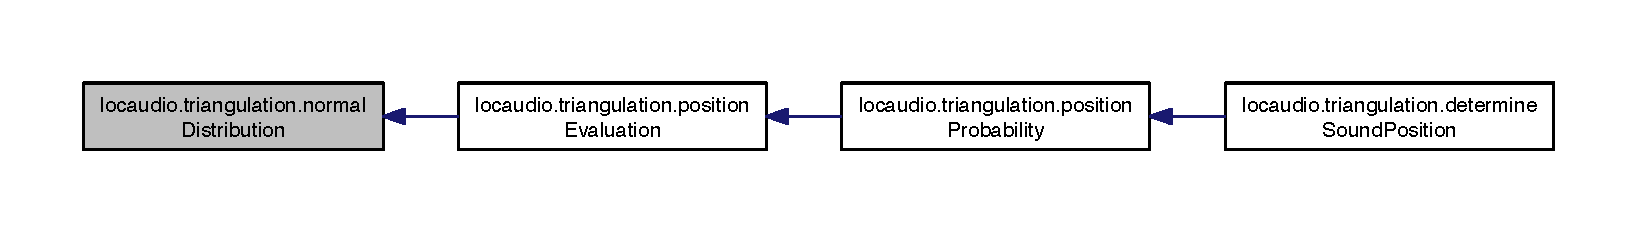
\includegraphics[width=350pt]{namespacelocaudio_1_1triangulation_aeda79115af2a41e618d834fe29a63104_icgraph}
\end{center}
\end{figure}


\hypertarget{namespacelocaudio_1_1triangulation_af600bbadd299c94825b159b5df236f6f}{\index{locaudio\-::triangulation@{locaudio\-::triangulation}!position\-Evaluation@{position\-Evaluation}}
\index{position\-Evaluation@{position\-Evaluation}!locaudio::triangulation@{locaudio\-::triangulation}}
\subsubsection[{position\-Evaluation}]{\setlength{\rightskip}{0pt plus 5cm}def locaudio.\-triangulation.\-position\-Evaluation (
\begin{DoxyParamCaption}
\item[{}]{x, }
\item[{}]{y, }
\item[{}]{r\-Ref, }
\item[{}]{l\-Ref, }
\item[{}]{node\-Events}
\end{DoxyParamCaption}
)}}\label{namespacelocaudio_1_1triangulation_af600bbadd299c94825b159b5df236f6f}


Evaluation function to deterimine with some weight, where a sound is located in the mesh network of nodes. 

Given an x and y, this returns a weight. The higher the weight, the higher the likelihood that the sound originated from x and y.


\begin{DoxyParams}{Parameters}
{\em x} & the horizontal location of the node event when the node event was captured\\
\hline
{\em y} & the vertical location of the node event when the node event was captured\\
\hline
{\em r\-Ref} & The reference distance at which the reference sound pressure level was recorded\\
\hline
{\em l\-Ref} & The reference sound pressure level used to determine the distance from the newly measured sound pressure level\\
\hline
{\em node\-Events} & The list ofassociated data when a node detects with some confidence that the sound has been identified\\
\hline
\end{DoxyParams}
\begin{DoxyReturn}{Returns}
The a result, given independent variables, x and y, and a configuration of node events with per sample sound constants, r\-Ref and l\-Ref, will be a value representing the likelihood of the sample sound being located at position (x, y). 
\end{DoxyReturn}


Definition at line 126 of file triangulation.\-py.



Here is the call graph for this function\-:\nopagebreak
\begin{figure}[H]
\begin{center}
\leavevmode
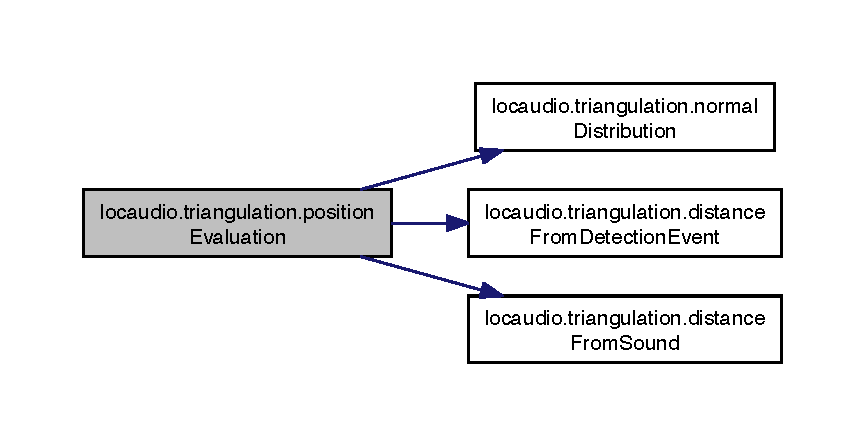
\includegraphics[width=350pt]{namespacelocaudio_1_1triangulation_af600bbadd299c94825b159b5df236f6f_cgraph}
\end{center}
\end{figure}




Here is the caller graph for this function\-:\nopagebreak
\begin{figure}[H]
\begin{center}
\leavevmode
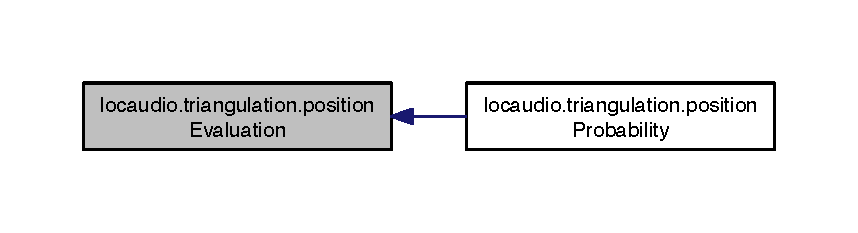
\includegraphics[width=350pt]{namespacelocaudio_1_1triangulation_af600bbadd299c94825b159b5df236f6f_icgraph}
\end{center}
\end{figure}


\hypertarget{namespacelocaudio_1_1triangulation_af708227f069b847392f730d13060cce8}{\index{locaudio\-::triangulation@{locaudio\-::triangulation}!position\-Probability@{position\-Probability}}
\index{position\-Probability@{position\-Probability}!locaudio::triangulation@{locaudio\-::triangulation}}
\subsubsection[{position\-Probability}]{\setlength{\rightskip}{0pt plus 5cm}def locaudio.\-triangulation.\-position\-Probability (
\begin{DoxyParamCaption}
\item[{}]{x, }
\item[{}]{y, }
\item[{}]{r\-Ref, }
\item[{}]{l\-Ref, }
\item[{}]{node\-Events}
\end{DoxyParamCaption}
)}}\label{namespacelocaudio_1_1triangulation_af708227f069b847392f730d13060cce8}


Scales the evaluation function so it returns a probability (i.\-e. 

a float between 0 and 1 inclusive) that a given x and y is where a sample sound originated from


\begin{DoxyParams}{Parameters}
{\em x} & the horizontal location of the node event when the node event was captured\\
\hline
{\em y} & the vertical location of the node event when the node event was captured\\
\hline
{\em r\-Ref} & The reference distance at which the reference sound pressure level was recorded\\
\hline
{\em l\-Ref} & The reference sound pressure level used to determine the distance from the newly measured sound pressure level\\
\hline
{\em node\-Events} & The list ofassociated data when a node detects with some confidence that the sound has been identified\\
\hline
\end{DoxyParams}
\begin{DoxyReturn}{Returns}
The a result, given independent variables, x and y, and a configuration of node events with per sample sound constants, r\-Ref and l\-Ref, will be a value representing the probability of the sample sound being located at position (x, y). 
\end{DoxyReturn}


Definition at line 168 of file triangulation.\-py.



Here is the call graph for this function\-:\nopagebreak
\begin{figure}[H]
\begin{center}
\leavevmode
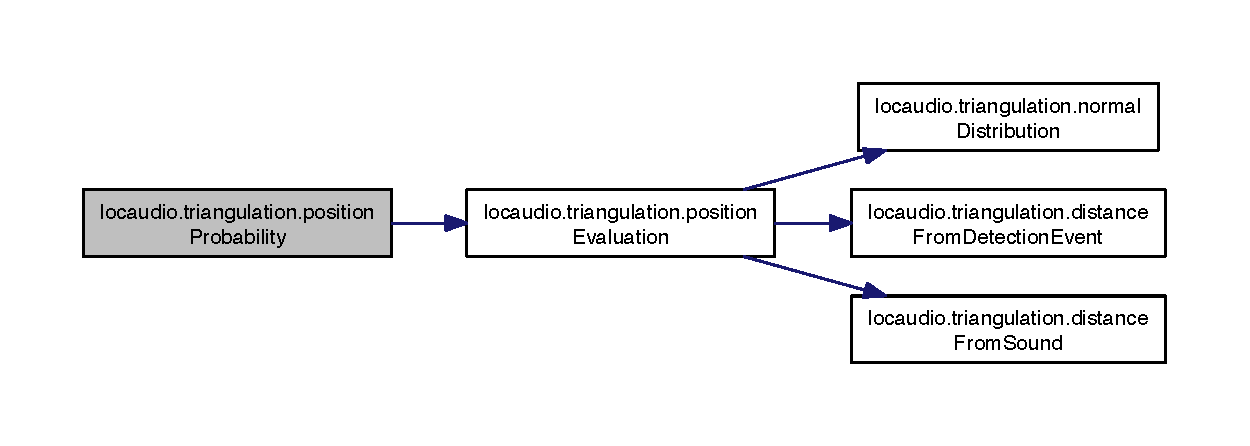
\includegraphics[width=350pt]{namespacelocaudio_1_1triangulation_af708227f069b847392f730d13060cce8_cgraph}
\end{center}
\end{figure}




Here is the caller graph for this function\-:\nopagebreak
\begin{figure}[H]
\begin{center}
\leavevmode
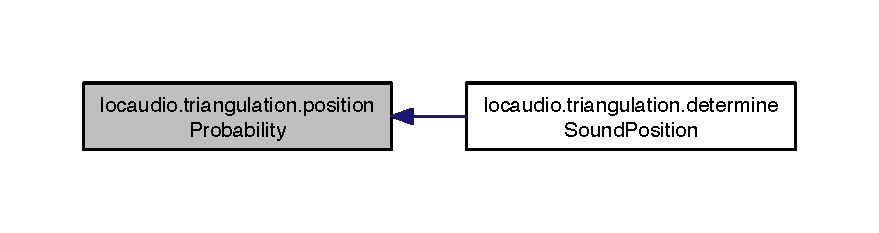
\includegraphics[width=350pt]{namespacelocaudio_1_1triangulation_af708227f069b847392f730d13060cce8_icgraph}
\end{center}
\end{figure}




\subsection{Variable Documentation}
\hypertarget{namespacelocaudio_1_1triangulation_ac85bcbed961d15baa586ddc0192860bb}{\index{locaudio\-::triangulation@{locaudio\-::triangulation}!K@{K}}
\index{K@{K}!locaudio::triangulation@{locaudio\-::triangulation}}
\subsubsection[{K}]{\setlength{\rightskip}{0pt plus 5cm}float locaudio.\-triangulation.\-K = 0.\-7}}\label{namespacelocaudio_1_1triangulation_ac85bcbed961d15baa586ddc0192860bb}


Scaling constant to transform a confidence probability into a a standard deviation. 



Definition at line 30 of file triangulation.\-py.


\chapter{Class Documentation}
\hypertarget{classlocaudio_1_1detectionevent_1_1DetectionEvent}{\section{locaudio.\-detectionevent.\-Detection\-Event Class Reference}
\label{classlocaudio_1_1detectionevent_1_1DetectionEvent}\index{locaudio.\-detectionevent.\-Detection\-Event@{locaudio.\-detectionevent.\-Detection\-Event}}
}


Class which is used to house the detection event.  




Inheritance diagram for locaudio.\-detectionevent.\-Detection\-Event\-:\nopagebreak
\begin{figure}[H]
\begin{center}
\leavevmode
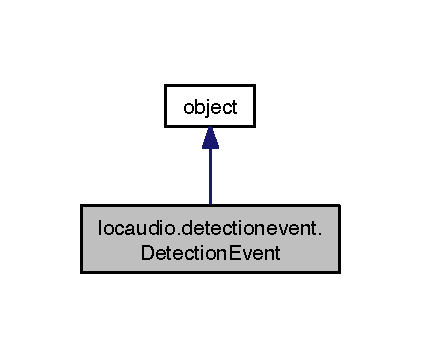
\includegraphics[width=202pt]{classlocaudio_1_1detectionevent_1_1DetectionEvent__inherit__graph}
\end{center}
\end{figure}


Collaboration diagram for locaudio.\-detectionevent.\-Detection\-Event\-:\nopagebreak
\begin{figure}[H]
\begin{center}
\leavevmode
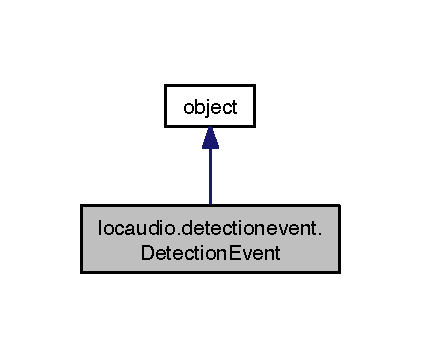
\includegraphics[width=202pt]{classlocaudio_1_1detectionevent_1_1DetectionEvent__coll__graph}
\end{center}
\end{figure}
\subsection*{Public Member Functions}
\begin{DoxyCompactItemize}
\item 
def \hyperlink{classlocaudio_1_1detectionevent_1_1DetectionEvent_aa998c7524a9484b5a3a7f80d4eba2280}{\-\_\-\-\_\-init\-\_\-\-\_\-}
\item 
def \hyperlink{classlocaudio_1_1detectionevent_1_1DetectionEvent_a220bfcacc5815c88912fe5fdc7b7a41c}{get\-\_\-x}
\item 
def \hyperlink{classlocaudio_1_1detectionevent_1_1DetectionEvent_a33b86d111b0979e20894dd7035aafb15}{get\-\_\-y}
\item 
def \hyperlink{classlocaudio_1_1detectionevent_1_1DetectionEvent_ae0e6b0c991471cfaf025d09c8730b45e}{get\-\_\-confidence}
\item 
def \hyperlink{classlocaudio_1_1detectionevent_1_1DetectionEvent_aa71a820d885f97dfb7aad1e32921cc75}{get\-\_\-spl}
\end{DoxyCompactItemize}
\subsection*{Public Attributes}
\begin{DoxyCompactItemize}
\item 
\hyperlink{classlocaudio_1_1detectionevent_1_1DetectionEvent_ae36950069a6f55e1f6e0251dbe80b0d4}{x}
\item 
\hyperlink{classlocaudio_1_1detectionevent_1_1DetectionEvent_aab867d871d3ab2bc608936ab64051b56}{y}
\item 
\hyperlink{classlocaudio_1_1detectionevent_1_1DetectionEvent_af0b955e105202f670cee964ce52d911f}{confidence}
\item 
\hyperlink{classlocaudio_1_1detectionevent_1_1DetectionEvent_aba6f9b944aea803742ef4aed6e34f215}{spl}
\end{DoxyCompactItemize}


\subsection{Detailed Description}
Class which is used to house the detection event. 

It is a persistent class which has variables x and y for position of the node when the event was registered, a confidence of sound recognition, and the sound pressure leve which can be used to determine the distance from the sound source. 

Definition at line 11 of file detectionevent.\-py.



\subsection{Constructor \& Destructor Documentation}
\hypertarget{classlocaudio_1_1detectionevent_1_1DetectionEvent_aa998c7524a9484b5a3a7f80d4eba2280}{\index{locaudio\-::detectionevent\-::\-Detection\-Event@{locaudio\-::detectionevent\-::\-Detection\-Event}!\-\_\-\-\_\-init\-\_\-\-\_\-@{\-\_\-\-\_\-init\-\_\-\-\_\-}}
\index{\-\_\-\-\_\-init\-\_\-\-\_\-@{\-\_\-\-\_\-init\-\_\-\-\_\-}!locaudio::detectionevent::DetectionEvent@{locaudio\-::detectionevent\-::\-Detection\-Event}}
\subsubsection[{\-\_\-\-\_\-init\-\_\-\-\_\-}]{\setlength{\rightskip}{0pt plus 5cm}def locaudio.\-detectionevent.\-Detection\-Event.\-\_\-\-\_\-init\-\_\-\-\_\- (
\begin{DoxyParamCaption}
\item[{}]{self, }
\item[{}]{x, }
\item[{}]{y, }
\item[{}]{confidence, }
\item[{}]{spl}
\end{DoxyParamCaption}
)}}\label{classlocaudio_1_1detectionevent_1_1DetectionEvent_aa998c7524a9484b5a3a7f80d4eba2280}


Definition at line 13 of file detectionevent.\-py.



\subsection{Member Function Documentation}
\hypertarget{classlocaudio_1_1detectionevent_1_1DetectionEvent_ae0e6b0c991471cfaf025d09c8730b45e}{\index{locaudio\-::detectionevent\-::\-Detection\-Event@{locaudio\-::detectionevent\-::\-Detection\-Event}!get\-\_\-confidence@{get\-\_\-confidence}}
\index{get\-\_\-confidence@{get\-\_\-confidence}!locaudio::detectionevent::DetectionEvent@{locaudio\-::detectionevent\-::\-Detection\-Event}}
\subsubsection[{get\-\_\-confidence}]{\setlength{\rightskip}{0pt plus 5cm}def locaudio.\-detectionevent.\-Detection\-Event.\-get\-\_\-confidence (
\begin{DoxyParamCaption}
\item[{}]{self}
\end{DoxyParamCaption}
)}}\label{classlocaudio_1_1detectionevent_1_1DetectionEvent_ae0e6b0c991471cfaf025d09c8730b45e}


Definition at line 28 of file detectionevent.\-py.

\hypertarget{classlocaudio_1_1detectionevent_1_1DetectionEvent_aa71a820d885f97dfb7aad1e32921cc75}{\index{locaudio\-::detectionevent\-::\-Detection\-Event@{locaudio\-::detectionevent\-::\-Detection\-Event}!get\-\_\-spl@{get\-\_\-spl}}
\index{get\-\_\-spl@{get\-\_\-spl}!locaudio::detectionevent::DetectionEvent@{locaudio\-::detectionevent\-::\-Detection\-Event}}
\subsubsection[{get\-\_\-spl}]{\setlength{\rightskip}{0pt plus 5cm}def locaudio.\-detectionevent.\-Detection\-Event.\-get\-\_\-spl (
\begin{DoxyParamCaption}
\item[{}]{self}
\end{DoxyParamCaption}
)}}\label{classlocaudio_1_1detectionevent_1_1DetectionEvent_aa71a820d885f97dfb7aad1e32921cc75}


Definition at line 31 of file detectionevent.\-py.

\hypertarget{classlocaudio_1_1detectionevent_1_1DetectionEvent_a220bfcacc5815c88912fe5fdc7b7a41c}{\index{locaudio\-::detectionevent\-::\-Detection\-Event@{locaudio\-::detectionevent\-::\-Detection\-Event}!get\-\_\-x@{get\-\_\-x}}
\index{get\-\_\-x@{get\-\_\-x}!locaudio::detectionevent::DetectionEvent@{locaudio\-::detectionevent\-::\-Detection\-Event}}
\subsubsection[{get\-\_\-x}]{\setlength{\rightskip}{0pt plus 5cm}def locaudio.\-detectionevent.\-Detection\-Event.\-get\-\_\-x (
\begin{DoxyParamCaption}
\item[{}]{self}
\end{DoxyParamCaption}
)}}\label{classlocaudio_1_1detectionevent_1_1DetectionEvent_a220bfcacc5815c88912fe5fdc7b7a41c}


Definition at line 20 of file detectionevent.\-py.

\hypertarget{classlocaudio_1_1detectionevent_1_1DetectionEvent_a33b86d111b0979e20894dd7035aafb15}{\index{locaudio\-::detectionevent\-::\-Detection\-Event@{locaudio\-::detectionevent\-::\-Detection\-Event}!get\-\_\-y@{get\-\_\-y}}
\index{get\-\_\-y@{get\-\_\-y}!locaudio::detectionevent::DetectionEvent@{locaudio\-::detectionevent\-::\-Detection\-Event}}
\subsubsection[{get\-\_\-y}]{\setlength{\rightskip}{0pt plus 5cm}def locaudio.\-detectionevent.\-Detection\-Event.\-get\-\_\-y (
\begin{DoxyParamCaption}
\item[{}]{self}
\end{DoxyParamCaption}
)}}\label{classlocaudio_1_1detectionevent_1_1DetectionEvent_a33b86d111b0979e20894dd7035aafb15}


Definition at line 24 of file detectionevent.\-py.



\subsection{Member Data Documentation}
\hypertarget{classlocaudio_1_1detectionevent_1_1DetectionEvent_af0b955e105202f670cee964ce52d911f}{\index{locaudio\-::detectionevent\-::\-Detection\-Event@{locaudio\-::detectionevent\-::\-Detection\-Event}!confidence@{confidence}}
\index{confidence@{confidence}!locaudio::detectionevent::DetectionEvent@{locaudio\-::detectionevent\-::\-Detection\-Event}}
\subsubsection[{confidence}]{\setlength{\rightskip}{0pt plus 5cm}locaudio.\-detectionevent.\-Detection\-Event.\-confidence}}\label{classlocaudio_1_1detectionevent_1_1DetectionEvent_af0b955e105202f670cee964ce52d911f}


Definition at line 16 of file detectionevent.\-py.

\hypertarget{classlocaudio_1_1detectionevent_1_1DetectionEvent_aba6f9b944aea803742ef4aed6e34f215}{\index{locaudio\-::detectionevent\-::\-Detection\-Event@{locaudio\-::detectionevent\-::\-Detection\-Event}!spl@{spl}}
\index{spl@{spl}!locaudio::detectionevent::DetectionEvent@{locaudio\-::detectionevent\-::\-Detection\-Event}}
\subsubsection[{spl}]{\setlength{\rightskip}{0pt plus 5cm}locaudio.\-detectionevent.\-Detection\-Event.\-spl}}\label{classlocaudio_1_1detectionevent_1_1DetectionEvent_aba6f9b944aea803742ef4aed6e34f215}


Definition at line 17 of file detectionevent.\-py.

\hypertarget{classlocaudio_1_1detectionevent_1_1DetectionEvent_ae36950069a6f55e1f6e0251dbe80b0d4}{\index{locaudio\-::detectionevent\-::\-Detection\-Event@{locaudio\-::detectionevent\-::\-Detection\-Event}!x@{x}}
\index{x@{x}!locaudio::detectionevent::DetectionEvent@{locaudio\-::detectionevent\-::\-Detection\-Event}}
\subsubsection[{x}]{\setlength{\rightskip}{0pt plus 5cm}locaudio.\-detectionevent.\-Detection\-Event.\-x}}\label{classlocaudio_1_1detectionevent_1_1DetectionEvent_ae36950069a6f55e1f6e0251dbe80b0d4}


Definition at line 14 of file detectionevent.\-py.

\hypertarget{classlocaudio_1_1detectionevent_1_1DetectionEvent_aab867d871d3ab2bc608936ab64051b56}{\index{locaudio\-::detectionevent\-::\-Detection\-Event@{locaudio\-::detectionevent\-::\-Detection\-Event}!y@{y}}
\index{y@{y}!locaudio::detectionevent::DetectionEvent@{locaudio\-::detectionevent\-::\-Detection\-Event}}
\subsubsection[{y}]{\setlength{\rightskip}{0pt plus 5cm}locaudio.\-detectionevent.\-Detection\-Event.\-y}}\label{classlocaudio_1_1detectionevent_1_1DetectionEvent_aab867d871d3ab2bc608936ab64051b56}


Definition at line 15 of file detectionevent.\-py.



The documentation for this class was generated from the following file\-:\begin{DoxyCompactItemize}
\item 
locaudio/\hyperlink{detectionevent_8py}{detectionevent.\-py}\end{DoxyCompactItemize}

\hypertarget{classlocaudio_1_1api_1_1Locaudio}{\section{locaudio.\-api.\-Locaudio Class Reference}
\label{classlocaudio_1_1api_1_1Locaudio}\index{locaudio.\-api.\-Locaudio@{locaudio.\-api.\-Locaudio}}
}
\subsection*{Public Member Functions}
\begin{DoxyCompactItemize}
\item 
def \hyperlink{classlocaudio_1_1api_1_1Locaudio_ab2d3bb5e705cb658077710485818b5f3}{\-\_\-\-\_\-init\-\_\-\-\_\-}
\item 
def \hyperlink{classlocaudio_1_1api_1_1Locaudio_a6b844b620c519b5b1726a271d004e92c}{get\-\_\-sound\-\_\-positions\-\_\-no\-\_\-block}
\item 
def \hyperlink{classlocaudio_1_1api_1_1Locaudio_a08eef102407125b656e6043c3bbfb756}{get\-\_\-sound\-\_\-positions}
\item 
def \hyperlink{classlocaudio_1_1api_1_1Locaudio_a463c89369ac3d0ccf2551c32a9b5ee91}{notify\-\_\-event}
\end{DoxyCompactItemize}
\subsection*{Public Attributes}
\begin{DoxyCompactItemize}
\item 
\hyperlink{classlocaudio_1_1api_1_1Locaudio_a97b12a0e2f549ea2d080e53d56609dfa}{url}
\item 
\hyperlink{classlocaudio_1_1api_1_1Locaudio_a36f2ab54cdc3581dc6f37d0731729b96}{pos\-\_\-url}
\item 
\hyperlink{classlocaudio_1_1api_1_1Locaudio_a6bf069251731e91dd2bdd291787b3e17}{notify\-\_\-url}
\item 
\hyperlink{classlocaudio_1_1api_1_1Locaudio_a0b5d0065ae0183383514e0ba1ed1858f}{sleep\-\_\-time}
\end{DoxyCompactItemize}


\subsection{Detailed Description}


Definition at line 8 of file api.\-py.



\subsection{Constructor \& Destructor Documentation}
\hypertarget{classlocaudio_1_1api_1_1Locaudio_ab2d3bb5e705cb658077710485818b5f3}{\index{locaudio\-::api\-::\-Locaudio@{locaudio\-::api\-::\-Locaudio}!\-\_\-\-\_\-init\-\_\-\-\_\-@{\-\_\-\-\_\-init\-\_\-\-\_\-}}
\index{\-\_\-\-\_\-init\-\_\-\-\_\-@{\-\_\-\-\_\-init\-\_\-\-\_\-}!locaudio::api::Locaudio@{locaudio\-::api\-::\-Locaudio}}
\subsubsection[{\-\_\-\-\_\-init\-\_\-\-\_\-}]{\setlength{\rightskip}{0pt plus 5cm}def locaudio.\-api.\-Locaudio.\-\_\-\-\_\-init\-\_\-\-\_\- (
\begin{DoxyParamCaption}
\item[{}]{self, }
\item[{}]{host, }
\item[{}]{port}
\end{DoxyParamCaption}
)}}\label{classlocaudio_1_1api_1_1Locaudio_ab2d3bb5e705cb658077710485818b5f3}


Definition at line 10 of file api.\-py.



\subsection{Member Function Documentation}
\hypertarget{classlocaudio_1_1api_1_1Locaudio_a08eef102407125b656e6043c3bbfb756}{\index{locaudio\-::api\-::\-Locaudio@{locaudio\-::api\-::\-Locaudio}!get\-\_\-sound\-\_\-positions@{get\-\_\-sound\-\_\-positions}}
\index{get\-\_\-sound\-\_\-positions@{get\-\_\-sound\-\_\-positions}!locaudio::api::Locaudio@{locaudio\-::api\-::\-Locaudio}}
\subsubsection[{get\-\_\-sound\-\_\-positions}]{\setlength{\rightskip}{0pt plus 5cm}def locaudio.\-api.\-Locaudio.\-get\-\_\-sound\-\_\-positions (
\begin{DoxyParamCaption}
\item[{}]{self}
\end{DoxyParamCaption}
)}}\label{classlocaudio_1_1api_1_1Locaudio_a08eef102407125b656e6043c3bbfb756}


Definition at line 23 of file api.\-py.



Here is the call graph for this function\-:
\nopagebreak
\begin{figure}[H]
\begin{center}
\leavevmode
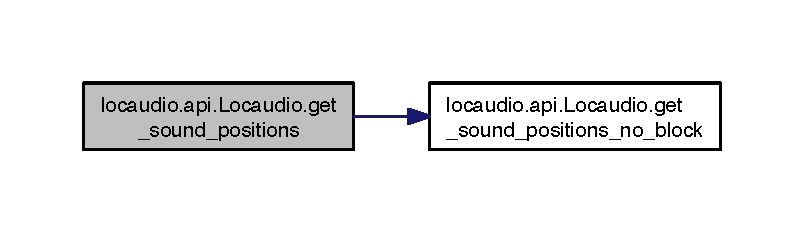
\includegraphics[width=350pt]{classlocaudio_1_1api_1_1Locaudio_a08eef102407125b656e6043c3bbfb756_cgraph}
\end{center}
\end{figure}


\hypertarget{classlocaudio_1_1api_1_1Locaudio_a6b844b620c519b5b1726a271d004e92c}{\index{locaudio\-::api\-::\-Locaudio@{locaudio\-::api\-::\-Locaudio}!get\-\_\-sound\-\_\-positions\-\_\-no\-\_\-block@{get\-\_\-sound\-\_\-positions\-\_\-no\-\_\-block}}
\index{get\-\_\-sound\-\_\-positions\-\_\-no\-\_\-block@{get\-\_\-sound\-\_\-positions\-\_\-no\-\_\-block}!locaudio::api::Locaudio@{locaudio\-::api\-::\-Locaudio}}
\subsubsection[{get\-\_\-sound\-\_\-positions\-\_\-no\-\_\-block}]{\setlength{\rightskip}{0pt plus 5cm}def locaudio.\-api.\-Locaudio.\-get\-\_\-sound\-\_\-positions\-\_\-no\-\_\-block (
\begin{DoxyParamCaption}
\item[{}]{self}
\end{DoxyParamCaption}
)}}\label{classlocaudio_1_1api_1_1Locaudio_a6b844b620c519b5b1726a271d004e92c}


Definition at line 17 of file api.\-py.



Here is the caller graph for this function\-:
\nopagebreak
\begin{figure}[H]
\begin{center}
\leavevmode
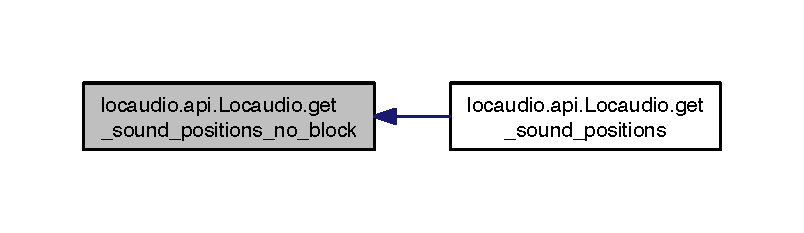
\includegraphics[width=350pt]{classlocaudio_1_1api_1_1Locaudio_a6b844b620c519b5b1726a271d004e92c_icgraph}
\end{center}
\end{figure}


\hypertarget{classlocaudio_1_1api_1_1Locaudio_a463c89369ac3d0ccf2551c32a9b5ee91}{\index{locaudio\-::api\-::\-Locaudio@{locaudio\-::api\-::\-Locaudio}!notify\-\_\-event@{notify\-\_\-event}}
\index{notify\-\_\-event@{notify\-\_\-event}!locaudio::api::Locaudio@{locaudio\-::api\-::\-Locaudio}}
\subsubsection[{notify\-\_\-event}]{\setlength{\rightskip}{0pt plus 5cm}def locaudio.\-api.\-Locaudio.\-notify\-\_\-event (
\begin{DoxyParamCaption}
\item[{}]{self, }
\item[{}]{data}
\end{DoxyParamCaption}
)}}\label{classlocaudio_1_1api_1_1Locaudio_a463c89369ac3d0ccf2551c32a9b5ee91}


Definition at line 32 of file api.\-py.



\subsection{Member Data Documentation}
\hypertarget{classlocaudio_1_1api_1_1Locaudio_a6bf069251731e91dd2bdd291787b3e17}{\index{locaudio\-::api\-::\-Locaudio@{locaudio\-::api\-::\-Locaudio}!notify\-\_\-url@{notify\-\_\-url}}
\index{notify\-\_\-url@{notify\-\_\-url}!locaudio::api::Locaudio@{locaudio\-::api\-::\-Locaudio}}
\subsubsection[{notify\-\_\-url}]{\setlength{\rightskip}{0pt plus 5cm}locaudio.\-api.\-Locaudio.\-notify\-\_\-url}}\label{classlocaudio_1_1api_1_1Locaudio_a6bf069251731e91dd2bdd291787b3e17}


Definition at line 13 of file api.\-py.

\hypertarget{classlocaudio_1_1api_1_1Locaudio_a36f2ab54cdc3581dc6f37d0731729b96}{\index{locaudio\-::api\-::\-Locaudio@{locaudio\-::api\-::\-Locaudio}!pos\-\_\-url@{pos\-\_\-url}}
\index{pos\-\_\-url@{pos\-\_\-url}!locaudio::api::Locaudio@{locaudio\-::api\-::\-Locaudio}}
\subsubsection[{pos\-\_\-url}]{\setlength{\rightskip}{0pt plus 5cm}locaudio.\-api.\-Locaudio.\-pos\-\_\-url}}\label{classlocaudio_1_1api_1_1Locaudio_a36f2ab54cdc3581dc6f37d0731729b96}


Definition at line 12 of file api.\-py.

\hypertarget{classlocaudio_1_1api_1_1Locaudio_a0b5d0065ae0183383514e0ba1ed1858f}{\index{locaudio\-::api\-::\-Locaudio@{locaudio\-::api\-::\-Locaudio}!sleep\-\_\-time@{sleep\-\_\-time}}
\index{sleep\-\_\-time@{sleep\-\_\-time}!locaudio::api::Locaudio@{locaudio\-::api\-::\-Locaudio}}
\subsubsection[{sleep\-\_\-time}]{\setlength{\rightskip}{0pt plus 5cm}locaudio.\-api.\-Locaudio.\-sleep\-\_\-time}}\label{classlocaudio_1_1api_1_1Locaudio_a0b5d0065ae0183383514e0ba1ed1858f}


Definition at line 14 of file api.\-py.

\hypertarget{classlocaudio_1_1api_1_1Locaudio_a97b12a0e2f549ea2d080e53d56609dfa}{\index{locaudio\-::api\-::\-Locaudio@{locaudio\-::api\-::\-Locaudio}!url@{url}}
\index{url@{url}!locaudio::api::Locaudio@{locaudio\-::api\-::\-Locaudio}}
\subsubsection[{url}]{\setlength{\rightskip}{0pt plus 5cm}locaudio.\-api.\-Locaudio.\-url}}\label{classlocaudio_1_1api_1_1Locaudio_a97b12a0e2f549ea2d080e53d56609dfa}


Definition at line 11 of file api.\-py.



The documentation for this class was generated from the following file\-:\begin{DoxyCompactItemize}
\item 
/\-Users/wallarelvo-\/mac/\-Documents/\-Projects/locaudio/locaudio/\hyperlink{api_8py}{api.\-py}\end{DoxyCompactItemize}

\hypertarget{classobject}{\section{object Class Reference}
\label{classobject}\index{object@{object}}
}


Inheritance diagram for object\-:
\nopagebreak
\begin{figure}[H]
\begin{center}
\leavevmode
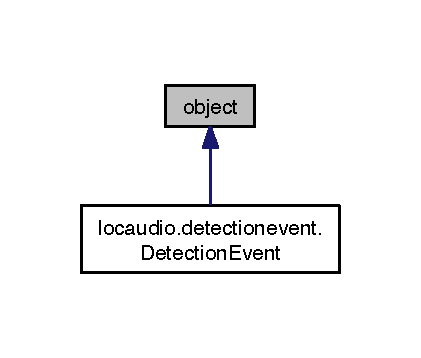
\includegraphics[width=324pt]{classobject__inherit__graph}
\end{center}
\end{figure}


The documentation for this class was generated from the following file\-:\begin{DoxyCompactItemize}
\item 
/\-Users/wallarelvo-\/mac/\-Documents/\-Projects/locaudio/locaudio/\hyperlink{detectionevent_8py}{detectionevent.\-py}\end{DoxyCompactItemize}

\hypertarget{classlocaudio_1_1point_1_1Point}{\section{locaudio.\-point.\-Point Class Reference}
\label{classlocaudio_1_1point_1_1Point}\index{locaudio.\-point.\-Point@{locaudio.\-point.\-Point}}
}


Inheritance diagram for locaudio.\-point.\-Point\-:
\nopagebreak
\begin{figure}[H]
\begin{center}
\leavevmode
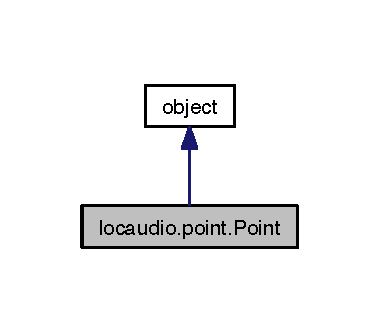
\includegraphics[width=182pt]{classlocaudio_1_1point_1_1Point__inherit__graph}
\end{center}
\end{figure}


Collaboration diagram for locaudio.\-point.\-Point\-:
\nopagebreak
\begin{figure}[H]
\begin{center}
\leavevmode
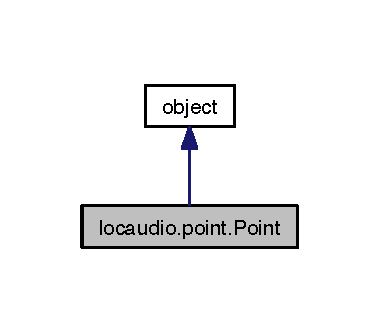
\includegraphics[width=182pt]{classlocaudio_1_1point_1_1Point__coll__graph}
\end{center}
\end{figure}
\subsection*{Public Member Functions}
\begin{DoxyCompactItemize}
\item 
def \hyperlink{classlocaudio_1_1point_1_1Point_a623c5e1c413d4e9ad61a670df2df3c7d}{\-\_\-\-\_\-init\-\_\-\-\_\-}
\item 
def \hyperlink{classlocaudio_1_1point_1_1Point_aed3cdb69eb0947bd839a5f58658a4ec8}{get\-\_\-x}
\item 
def \hyperlink{classlocaudio_1_1point_1_1Point_abbb24f2a2b4a776a81c755044d3d3c1d}{get\-\_\-y}
\item 
def \hyperlink{classlocaudio_1_1point_1_1Point_a321adfaa5bbe604f7d95e8d3453728f5}{set\-\_\-x}
\item 
def \hyperlink{classlocaudio_1_1point_1_1Point_a09e41fa59a48f850881cd13f923324d3}{set\-\_\-y}
\item 
def \hyperlink{classlocaudio_1_1point_1_1Point_aa1ed49a30a5e6589c8752530f261f9dd}{to\-\_\-list}
\item 
def \hyperlink{classlocaudio_1_1point_1_1Point_afd4dda0197e7d2a6853238294cb4ce93}{\-\_\-\-\_\-repr\-\_\-\-\_\-}
\end{DoxyCompactItemize}
\subsection*{Public Attributes}
\begin{DoxyCompactItemize}
\item 
\hyperlink{classlocaudio_1_1point_1_1Point_a6ff592bd2d87595950205335419de676}{x}
\item 
\hyperlink{classlocaudio_1_1point_1_1Point_a714d448f12192ca6d947e7109fb8f538}{y}
\end{DoxyCompactItemize}


\subsection{Detailed Description}


Definition at line 2 of file point.\-py.



\subsection{Constructor \& Destructor Documentation}
\hypertarget{classlocaudio_1_1point_1_1Point_a623c5e1c413d4e9ad61a670df2df3c7d}{\index{locaudio\-::point\-::\-Point@{locaudio\-::point\-::\-Point}!\-\_\-\-\_\-init\-\_\-\-\_\-@{\-\_\-\-\_\-init\-\_\-\-\_\-}}
\index{\-\_\-\-\_\-init\-\_\-\-\_\-@{\-\_\-\-\_\-init\-\_\-\-\_\-}!locaudio::point::Point@{locaudio\-::point\-::\-Point}}
\subsubsection[{\-\_\-\-\_\-init\-\_\-\-\_\-}]{\setlength{\rightskip}{0pt plus 5cm}def locaudio.\-point.\-Point.\-\_\-\-\_\-init\-\_\-\-\_\- (
\begin{DoxyParamCaption}
\item[{}]{self, }
\item[{}]{x, }
\item[{}]{y}
\end{DoxyParamCaption}
)}}\label{classlocaudio_1_1point_1_1Point_a623c5e1c413d4e9ad61a670df2df3c7d}


Definition at line 4 of file point.\-py.



\subsection{Member Function Documentation}
\hypertarget{classlocaudio_1_1point_1_1Point_afd4dda0197e7d2a6853238294cb4ce93}{\index{locaudio\-::point\-::\-Point@{locaudio\-::point\-::\-Point}!\-\_\-\-\_\-repr\-\_\-\-\_\-@{\-\_\-\-\_\-repr\-\_\-\-\_\-}}
\index{\-\_\-\-\_\-repr\-\_\-\-\_\-@{\-\_\-\-\_\-repr\-\_\-\-\_\-}!locaudio::point::Point@{locaudio\-::point\-::\-Point}}
\subsubsection[{\-\_\-\-\_\-repr\-\_\-\-\_\-}]{\setlength{\rightskip}{0pt plus 5cm}def locaudio.\-point.\-Point.\-\_\-\-\_\-repr\-\_\-\-\_\- (
\begin{DoxyParamCaption}
\item[{}]{self}
\end{DoxyParamCaption}
)}}\label{classlocaudio_1_1point_1_1Point_afd4dda0197e7d2a6853238294cb4ce93}


Definition at line 31 of file point.\-py.

\hypertarget{classlocaudio_1_1point_1_1Point_aed3cdb69eb0947bd839a5f58658a4ec8}{\index{locaudio\-::point\-::\-Point@{locaudio\-::point\-::\-Point}!get\-\_\-x@{get\-\_\-x}}
\index{get\-\_\-x@{get\-\_\-x}!locaudio::point::Point@{locaudio\-::point\-::\-Point}}
\subsubsection[{get\-\_\-x}]{\setlength{\rightskip}{0pt plus 5cm}def locaudio.\-point.\-Point.\-get\-\_\-x (
\begin{DoxyParamCaption}
\item[{}]{self}
\end{DoxyParamCaption}
)}}\label{classlocaudio_1_1point_1_1Point_aed3cdb69eb0947bd839a5f58658a4ec8}


Definition at line 9 of file point.\-py.

\hypertarget{classlocaudio_1_1point_1_1Point_abbb24f2a2b4a776a81c755044d3d3c1d}{\index{locaudio\-::point\-::\-Point@{locaudio\-::point\-::\-Point}!get\-\_\-y@{get\-\_\-y}}
\index{get\-\_\-y@{get\-\_\-y}!locaudio::point::Point@{locaudio\-::point\-::\-Point}}
\subsubsection[{get\-\_\-y}]{\setlength{\rightskip}{0pt plus 5cm}def locaudio.\-point.\-Point.\-get\-\_\-y (
\begin{DoxyParamCaption}
\item[{}]{self}
\end{DoxyParamCaption}
)}}\label{classlocaudio_1_1point_1_1Point_abbb24f2a2b4a776a81c755044d3d3c1d}


Definition at line 13 of file point.\-py.

\hypertarget{classlocaudio_1_1point_1_1Point_a321adfaa5bbe604f7d95e8d3453728f5}{\index{locaudio\-::point\-::\-Point@{locaudio\-::point\-::\-Point}!set\-\_\-x@{set\-\_\-x}}
\index{set\-\_\-x@{set\-\_\-x}!locaudio::point::Point@{locaudio\-::point\-::\-Point}}
\subsubsection[{set\-\_\-x}]{\setlength{\rightskip}{0pt plus 5cm}def locaudio.\-point.\-Point.\-set\-\_\-x (
\begin{DoxyParamCaption}
\item[{}]{self, }
\item[{}]{x}
\end{DoxyParamCaption}
)}}\label{classlocaudio_1_1point_1_1Point_a321adfaa5bbe604f7d95e8d3453728f5}


Definition at line 17 of file point.\-py.

\hypertarget{classlocaudio_1_1point_1_1Point_a09e41fa59a48f850881cd13f923324d3}{\index{locaudio\-::point\-::\-Point@{locaudio\-::point\-::\-Point}!set\-\_\-y@{set\-\_\-y}}
\index{set\-\_\-y@{set\-\_\-y}!locaudio::point::Point@{locaudio\-::point\-::\-Point}}
\subsubsection[{set\-\_\-y}]{\setlength{\rightskip}{0pt plus 5cm}def locaudio.\-point.\-Point.\-set\-\_\-y (
\begin{DoxyParamCaption}
\item[{}]{self, }
\item[{}]{y}
\end{DoxyParamCaption}
)}}\label{classlocaudio_1_1point_1_1Point_a09e41fa59a48f850881cd13f923324d3}


Definition at line 22 of file point.\-py.

\hypertarget{classlocaudio_1_1point_1_1Point_aa1ed49a30a5e6589c8752530f261f9dd}{\index{locaudio\-::point\-::\-Point@{locaudio\-::point\-::\-Point}!to\-\_\-list@{to\-\_\-list}}
\index{to\-\_\-list@{to\-\_\-list}!locaudio::point::Point@{locaudio\-::point\-::\-Point}}
\subsubsection[{to\-\_\-list}]{\setlength{\rightskip}{0pt plus 5cm}def locaudio.\-point.\-Point.\-to\-\_\-list (
\begin{DoxyParamCaption}
\item[{}]{self}
\end{DoxyParamCaption}
)}}\label{classlocaudio_1_1point_1_1Point_aa1ed49a30a5e6589c8752530f261f9dd}


Definition at line 27 of file point.\-py.



\subsection{Member Data Documentation}
\hypertarget{classlocaudio_1_1point_1_1Point_a6ff592bd2d87595950205335419de676}{\index{locaudio\-::point\-::\-Point@{locaudio\-::point\-::\-Point}!x@{x}}
\index{x@{x}!locaudio::point::Point@{locaudio\-::point\-::\-Point}}
\subsubsection[{x}]{\setlength{\rightskip}{0pt plus 5cm}locaudio.\-point.\-Point.\-x}}\label{classlocaudio_1_1point_1_1Point_a6ff592bd2d87595950205335419de676}


Definition at line 5 of file point.\-py.

\hypertarget{classlocaudio_1_1point_1_1Point_a714d448f12192ca6d947e7109fb8f538}{\index{locaudio\-::point\-::\-Point@{locaudio\-::point\-::\-Point}!y@{y}}
\index{y@{y}!locaudio::point::Point@{locaudio\-::point\-::\-Point}}
\subsubsection[{y}]{\setlength{\rightskip}{0pt plus 5cm}locaudio.\-point.\-Point.\-y}}\label{classlocaudio_1_1point_1_1Point_a714d448f12192ca6d947e7109fb8f538}


Definition at line 6 of file point.\-py.



The documentation for this class was generated from the following file\-:\begin{DoxyCompactItemize}
\item 
/\-Users/wallarelvo-\/mac/\-Documents/\-Projects/locaudio/locaudio/\hyperlink{point_8py}{point.\-py}\end{DoxyCompactItemize}

\chapter{File Documentation}
\hypertarget{____init_____8py}{\section{locaudio/\-\_\-\-\_\-init\-\_\-\-\_\-.py File Reference}
\label{____init_____8py}\index{locaudio/\-\_\-\-\_\-init\-\_\-\-\_\-.\-py@{locaudio/\-\_\-\-\_\-init\-\_\-\-\_\-.\-py}}
}
\subsection*{Namespaces}
\begin{DoxyCompactItemize}
\item 
\hyperlink{namespacelocaudio}{locaudio}
\end{DoxyCompactItemize}
\subsection*{Constant Groups}
\begin{DoxyCompactItemize}
\item 
\hyperlink{namespacelocaudio}{locaudio}
\end{DoxyCompactItemize}
\subsection*{Variables}
\begin{DoxyCompactItemize}
\item 
string \hyperlink{namespacelocaudio_a08bd2e574ba3b2af29ee1231a056dcc5}{locaudio.\-\_\-\-\_\-author\-\_\-\-\_\-} = \char`\"{}Alexander Wallar $<$aw204@st-\/andrews.\-ac.\-uk$>$\char`\"{}
\end{DoxyCompactItemize}

\hypertarget{api_8py}{\section{/\-Users/wallarelvo-\/mac/\-Documents/\-Projects/locaudio/locaudio/api.py File Reference}
\label{api_8py}\index{/\-Users/wallarelvo-\/mac/\-Documents/\-Projects/locaudio/locaudio/api.\-py@{/\-Users/wallarelvo-\/mac/\-Documents/\-Projects/locaudio/locaudio/api.\-py}}
}
\subsection*{Classes}
\begin{DoxyCompactItemize}
\item 
class \hyperlink{classlocaudio_1_1api_1_1Locaudio}{locaudio.\-api.\-Locaudio}
\end{DoxyCompactItemize}
\subsection*{Namespaces}
\begin{DoxyCompactItemize}
\item 
\hyperlink{namespacelocaudio_1_1api}{locaudio.\-api}
\end{DoxyCompactItemize}
\subsection*{Constant Groups}
\begin{DoxyCompactItemize}
\item 
\hyperlink{namespacelocaudio_1_1api}{locaudio.\-api}
\end{DoxyCompactItemize}

\hypertarget{config_8py}{\section{/\-Users/wallarelvo-\/mac/\-Documents/\-Projects/locaudio/locaudio/config.py File Reference}
\label{config_8py}\index{/\-Users/wallarelvo-\/mac/\-Documents/\-Projects/locaudio/locaudio/config.\-py@{/\-Users/wallarelvo-\/mac/\-Documents/\-Projects/locaudio/locaudio/config.\-py}}
}
\subsection*{Namespaces}
\begin{DoxyCompactItemize}
\item 
\hyperlink{namespacelocaudio_1_1config}{locaudio.\-config}
\end{DoxyCompactItemize}
\subsection*{Constant Groups}
\begin{DoxyCompactItemize}
\item 
\hyperlink{namespacelocaudio_1_1config}{locaudio.\-config}
\end{DoxyCompactItemize}
\subsection*{Variables}
\begin{DoxyCompactItemize}
\item 
tuple \hyperlink{namespacelocaudio_1_1config_a360c0d0146f0defa6e852b004d834513}{locaudio.\-config.\-app} = Flask(\-\_\-\-\_\-name\-\_\-\-\_\-)
\item 
tuple \hyperlink{namespacelocaudio_1_1config_ac701fbe139aea54ed29426657c92739e}{locaudio.\-config.\-detection\-\_\-events} = list()
\item 
int \hyperlink{namespacelocaudio_1_1config_a7a507b1534e99737ed545a117b87313b}{locaudio.\-config.\-refresh\-\_\-time} = 10
\item 
\hyperlink{namespacelocaudio_1_1config_a6c08de266870244fd753c8dc6047bfec}{locaudio.\-config.\-reference\-\_\-print} = None
\item 
tuple \hyperlink{namespacelocaudio_1_1config_afc387e694f7bc08bccf873238760ce8e}{locaudio.\-config.\-position\-\_\-list} = list()
\item 
\hyperlink{namespacelocaudio_1_1config_aa8acdbffcae328560e4231de29c2dc1a}{locaudio.\-config.\-new\-\_\-data} = False
\end{DoxyCompactItemize}

\hypertarget{detectionevent_8py}{\section{/\-Users/wallarelvo-\/mac/\-Documents/\-Projects/locaudio/locaudio/detectionevent.py File Reference}
\label{detectionevent_8py}\index{/\-Users/wallarelvo-\/mac/\-Documents/\-Projects/locaudio/locaudio/detectionevent.\-py@{/\-Users/wallarelvo-\/mac/\-Documents/\-Projects/locaudio/locaudio/detectionevent.\-py}}
}
\subsection*{Classes}
\begin{DoxyCompactItemize}
\item 
class \hyperlink{classlocaudio_1_1detectionevent_1_1DetectionEvent}{locaudio.\-detectionevent.\-Detection\-Event}
\begin{DoxyCompactList}\small\item\em Class which is used to house the detection event. \end{DoxyCompactList}\end{DoxyCompactItemize}
\subsection*{Namespaces}
\begin{DoxyCompactItemize}
\item 
\hyperlink{namespacelocaudio_1_1detectionevent}{locaudio.\-detectionevent}
\end{DoxyCompactItemize}
\subsection*{Constant Groups}
\begin{DoxyCompactItemize}
\item 
\hyperlink{namespacelocaudio_1_1detectionevent}{locaudio.\-detectionevent}
\end{DoxyCompactItemize}

\hypertarget{detectionserver_8py}{\section{/\-Users/wallarelvo-\/mac/\-Documents/\-Projects/locaudio/locaudio/detectionserver.py File Reference}
\label{detectionserver_8py}\index{/\-Users/wallarelvo-\/mac/\-Documents/\-Projects/locaudio/locaudio/detectionserver.\-py@{/\-Users/wallarelvo-\/mac/\-Documents/\-Projects/locaudio/locaudio/detectionserver.\-py}}
}
\subsection*{Namespaces}
\begin{DoxyCompactItemize}
\item 
\hyperlink{namespacelocaudio_1_1detectionserver}{locaudio.\-detectionserver}
\end{DoxyCompactItemize}
\subsection*{Constant Groups}
\begin{DoxyCompactItemize}
\item 
\hyperlink{namespacelocaudio_1_1detectionserver}{locaudio.\-detectionserver}
\end{DoxyCompactItemize}
\subsection*{Functions}
\begin{DoxyCompactItemize}
\item 
def \hyperlink{namespacelocaudio_1_1detectionserver_a5191437c6dcef4900a200a7dd115a58a}{locaudio.\-detectionserver.\-post\-\_\-notify}
\end{DoxyCompactItemize}
\subsection*{Variables}
\begin{DoxyCompactItemize}
\item 
tuple \hyperlink{namespacelocaudio_1_1detectionserver_aef3614adbb1729e98db6ad1e92df44aa}{locaudio.\-detectionserver.\-app} = Flask(\-\_\-\-\_\-name\-\_\-\-\_\-)
\end{DoxyCompactItemize}

\hypertarget{fingerprint_8py}{\section{/\-Users/wallarelvo-\/mac/\-Documents/\-Projects/locaudio/locaudio/fingerprint.py File Reference}
\label{fingerprint_8py}\index{/\-Users/wallarelvo-\/mac/\-Documents/\-Projects/locaudio/locaudio/fingerprint.\-py@{/\-Users/wallarelvo-\/mac/\-Documents/\-Projects/locaudio/locaudio/fingerprint.\-py}}
}
\subsection*{Namespaces}
\begin{DoxyCompactItemize}
\item 
\hyperlink{namespacelocaudio_1_1fingerprint}{locaudio.\-fingerprint}
\end{DoxyCompactItemize}
\subsection*{Constant Groups}
\begin{DoxyCompactItemize}
\item 
\hyperlink{namespacelocaudio_1_1fingerprint}{locaudio.\-fingerprint}
\end{DoxyCompactItemize}
\subsection*{Functions}
\begin{DoxyCompactItemize}
\item 
def \hyperlink{namespacelocaudio_1_1fingerprint_aff6c231dfe74871cf275c4b8249fafb2}{locaudio.\-fingerprint.\-get\-\_\-similarity}
\end{DoxyCompactItemize}
\subsection*{Variables}
\begin{DoxyCompactItemize}
\item 
tuple \hyperlink{namespacelocaudio_1_1fingerprint_ad6f4abf7a6777721b881a7f0188afe92}{locaudio.\-fingerprint.\-Reference\-Print} = namedtuple(\char`\"{}Reference\-Print\char`\"{}, \char`\"{}fingerprint radius spl\char`\"{})
\end{DoxyCompactItemize}

\hypertarget{point_8py}{\section{/\-Users/wallarelvo-\/mac/\-Documents/\-Projects/locaudio/locaudio/point.py File Reference}
\label{point_8py}\index{/\-Users/wallarelvo-\/mac/\-Documents/\-Projects/locaudio/locaudio/point.\-py@{/\-Users/wallarelvo-\/mac/\-Documents/\-Projects/locaudio/locaudio/point.\-py}}
}
\subsection*{Classes}
\begin{DoxyCompactItemize}
\item 
class \hyperlink{classlocaudio_1_1point_1_1Point}{locaudio.\-point.\-Point}
\end{DoxyCompactItemize}
\subsection*{Namespaces}
\begin{DoxyCompactItemize}
\item 
\hyperlink{namespacelocaudio_1_1point}{locaudio.\-point}
\end{DoxyCompactItemize}
\subsection*{Constant Groups}
\begin{DoxyCompactItemize}
\item 
\hyperlink{namespacelocaudio_1_1point}{locaudio.\-point}
\end{DoxyCompactItemize}

\hypertarget{triangulation_8py}{\section{/\-Users/wallarelvo-\/mac/\-Documents/\-Projects/locaudio/locaudio/triangulation.py File Reference}
\label{triangulation_8py}\index{/\-Users/wallarelvo-\/mac/\-Documents/\-Projects/locaudio/locaudio/triangulation.\-py@{/\-Users/wallarelvo-\/mac/\-Documents/\-Projects/locaudio/locaudio/triangulation.\-py}}
}
\subsection*{Namespaces}
\begin{DoxyCompactItemize}
\item 
\hyperlink{namespacelocaudio_1_1triangulation}{locaudio.\-triangulation}
\end{DoxyCompactItemize}
\subsection*{Constant Groups}
\begin{DoxyCompactItemize}
\item 
\hyperlink{namespacelocaudio_1_1triangulation}{locaudio.\-triangulation}
\end{DoxyCompactItemize}
\subsection*{Functions}
\begin{DoxyCompactItemize}
\item 
def \hyperlink{namespacelocaudio_1_1triangulation_aa6072b3aad637ae71a38424f23014a86}{locaudio.\-triangulation.\-distance\-\_\-from\-\_\-sound}
\begin{DoxyCompactList}\small\item\em Determines the distance from a sound given the sound pressure level and a reference sound pressure level with an associated distance. \end{DoxyCompactList}\item 
def \hyperlink{namespacelocaudio_1_1triangulation_a1206790ce9fd39f59ce264ac7c7fb443}{locaudio.\-triangulation.\-distance\-\_\-from\-\_\-detection\-\_\-event}
\begin{DoxyCompactList}\small\item\em Given x and y coordinates, this returns the distance to a node\-Event where the node\-Event has attributes, x and y, on the same plane. \end{DoxyCompactList}\item 
def \hyperlink{namespacelocaudio_1_1triangulation_aa221cba0226b13aff028ca9155dfbd76}{locaudio.\-triangulation.\-normal\-\_\-distribution}
\begin{DoxyCompactList}\small\item\em This is the normal distribution function. \end{DoxyCompactList}\item 
def \hyperlink{namespacelocaudio_1_1triangulation_ad44e1bed6beed7ee59cffc4c230f7144}{locaudio.\-triangulation.\-set\-\_\-node\-\_\-events\-\_\-std}
\begin{DoxyCompactList}\small\item\em Uses the relative time differences between the node events mixed with the confidence of sound recognition to determine the standard deviation of the node event. \end{DoxyCompactList}\item 
def \hyperlink{namespacelocaudio_1_1triangulation_acf50f5be4536fb0929c359396d41828f}{locaudio.\-triangulation.\-position\-\_\-evaluation}
\begin{DoxyCompactList}\small\item\em Evaluation function to deterimine with some weight, where a sound is located in the mesh network of nodes. \end{DoxyCompactList}\item 
def \hyperlink{namespacelocaudio_1_1triangulation_ab85ddfec0f2c6c1c20134d90a6fe874a}{locaudio.\-triangulation.\-position\-\_\-probability}
\begin{DoxyCompactList}\small\item\em Scales the evaluation function so it returns a probability (i.\-e. \end{DoxyCompactList}\item 
def \hyperlink{namespacelocaudio_1_1triangulation_ad01abd5ed08c05988dea7978b141549c}{locaudio.\-triangulation.\-determine\-\_\-sound\-\_\-position\-\_\-list}
\begin{DoxyCompactList}\small\item\em Determines a list of possible positions of where the sound will be located. \end{DoxyCompactList}\item 
def \hyperlink{namespacelocaudio_1_1triangulation_aaf881f389e42011e1bacc2247794cc7d}{locaudio.\-triangulation.\-determine\-\_\-peaks}
\begin{DoxyCompactList}\small\item\em Given a list of \char`\"{}optimized\char`\"{} points and their corresponding probabilities and a list of labels returned from the clustering algorithm, this function goes through all of the optimized points and returns the ones with the highest probabilities and issues them as cluter centers. \end{DoxyCompactList}\item 
def \hyperlink{namespacelocaudio_1_1triangulation_a37420560e73cb3aefbdff181774725be}{locaudio.\-triangulation.\-determine\-\_\-sound\-\_\-positions}
\begin{DoxyCompactList}\small\item\em Determines the position in the probability grid that has the highest probability of being the position of the sound. \end{DoxyCompactList}\item 
def \hyperlink{namespacelocaudio_1_1triangulation_a91ab07f598b1161238e199e127fef855}{locaudio.\-triangulation.\-generate\-\_\-sound\-\_\-position\-\_\-func}
\begin{DoxyCompactList}\small\item\em This is a closure that provides a new function that makes it so the developer does not need to continue passing the r\-Ref, l\-Ref and init\-Guess variables when determining the sound position. \end{DoxyCompactList}\end{DoxyCompactItemize}
\subsection*{Variables}
\begin{DoxyCompactItemize}
\item 
float \hyperlink{namespacelocaudio_1_1triangulation_ac85bcbed961d15baa586ddc0192860bb}{locaudio.\-triangulation.\-K} = 0.\-7
\begin{DoxyCompactList}\small\item\em Scaling constant to transform a confidence probability into a a standard deviation. \end{DoxyCompactList}\end{DoxyCompactItemize}

%--- End generated contents ---

% Index
\newpage
\phantomsection
\addcontentsline{toc}{part}{Index}
\printindex

\end{document}
